\chapter{Systementwurf}
\label{systementwurf}
Im folgenden Kapitel werden die von CloudGrid verwendeten Komponenten, unter Beachtung der zuvor definierten Anforderungen, beschrieben.
Dazu wird zuerst die verwendete Programmierumgebung analysiert, da diese für die weiteren Abschnitte relevant sein wird.
Danach werden mögliche Cloudservices evaluiert und auf deren rechtliche Bedingungen eingegangen.
Darauf aufbauend wird die Architektur des Systems aufgezeigt und die einzelnen Schichten der Architektur des Systems beschrieben.

% #########################################################
% ################## Programmierumgebung ##################
\section{Programmierumgebung}
\label{systementwurf-programmierumgebung}
Die Wahl der Programmierumgebung ist maßgeblich für die Anwendung.
Dabei richtet sich sowohl die Umsetzung der Benutzeroberfläche, als auch die Wahl möglicher Plugins und Bibliotheken, nach selbiger.
Unter Berücksichtigung der Kriterien aus Abschnitt \ref{anforderungtech} wurden die folgenden Programmierumgebungen analysiert.

\paragraph{C:}
Die Vorteile von C liegen bei der Effizienz im Umgang mit dem Filesystem und der direkten Manipulation des Arbeitsspeichers.
Als Nachteil hingegen ist das Fehlen der objektorientierten Programmierung zu nennen.
Dadurch ist es schwieriger, sowohl den Quellcode modular aufzubauen, als auch für andere Entwickler eigene Module in die Anwendung zu integrieren.
Darüber hinaus gibt es nur wenige Bibliotheken zum Verarbeiten von \ac{HTTP} Requests.
Zudem ist die Lernkurve für die \ac{GUI} Entwicklung steil und erfordert fundiertes Vorwissen in der jeweiligen Bibliothek.
Ein weiterer Nachteil ist es, dass mit C keine plattformunabhängige Programmierung möglich ist.
Der Programmierer muss viele Sonderfälle berücksichtigen und somit Anpassungen für das jeweilige Zielsystem einbauen.

\paragraph{\cpp :}
Diese ist der Funktionsweise von C sehr ähnlich.
Dadurch entstehen ähnliche Vor- und Nachteile.
Beispielsweise arbeitet diese ähnlich effizient mit dem Filesystem, hat aber auch dieselben Nachteile was die plattformunabhängige Programmierung betrifft und eine ähnlich steile Lernkurve wie bei C.
Lediglich die Unterstützung von Objektorientierung ist als großer Vorteil zu vermerken.

\paragraph{Java:}
Anders als die beiden bisher vorgestellten Programmiersprachen, wird Java nicht direkt vom Betriebssystem ausgeführt, sondern in der Java Virtual Machine.
Der Vorteil dabei ist, dass die Sprache dadurch plattformunabhängig ist.
Jedoch gestaltet sich dadurch die Arbeit auf dem Filesystem als weniger effizient.
Zudem belegt die Java Virtual Machine sowohl erheblich viel Arbeitsspeicher, als auch Prozessorleistung, da sie zum Ausführen von Javaprogrammen mit gestartet und im Hintergrund ausgeführt wird.
Ähnlich wie \cpp\ ist Java objektorientiert, was die Erweiterung des Systems für Entwickler leichter macht.
Dank der Apache Commons\footnote{\url{http://commons.apache.org}}, einer Klassenbibliothek der Apache Inc., werden viele Standardfunktionen nachgeliefert.
Somit wird ein gutes \ac{HTTP} Handling und auch das Handling von OAuth Request ermöglicht.
Auf Seiten der \ac{GUI} gibt es die selben Probleme wie bei C und \cpp .

\paragraph{Node.js:}
Diese recht junge Entwicklungsumgebung, welche auf der Google JavaScript Engine V8\footnote{\url{https://code.google.com/p/v8}} basiert.
Diese ist in \cpp\ geschrieben, sodass Node.js damit letztendlich auf \cpp\ aufsetzt.
Das ermöglicht eine effiziente Bearbeitung des Filesystems und des Speicherzugriffs.
Ein Programm wird in JavaScript geschrieben, kann aber darüber hinaus über \cpp\ Module verfügen.
Node.js ist für alle gängigen Betriebssysteme, Windows, Mac OS X und Linux, verfügbar.
Der primäre Anwendungsbereich ist die Funktion als Webserver.
Jedoch lassen sich auch Desktopanwendungen damit umsetzen.
Durch die Webserverfunktionalität kann die \ac{GUI} der Anwendung komplett mit \ac{HTML} und \ac{CSS} im Browser umgesetzt werden.
Das gibt dem User eine gewohnte Arbeitsumgebung.
Node.js ist modular aufgebaut, sodass einzelne Plugins nachgeladen werden können.
Darüber hinaus können diese Plugins, sowie Node.js selbst, über ein einfaches Installationsskript bei dem Benutzer installiert werden.

\paragraph{Fazit:}
Unter Berücksichtigung der in Abschnitt \ref{anforderungtech} definierten Anforderungen und der in diesem Abschnitt evaluierten Programmierumgebungen, wird bei der Umsetzung von CloudGrid auf Node.js gesetzt.
Diese bietet die Vorteile einer effizienten Ausführung, wie beispielsweise \cpp\ und ermöglicht darüber hinaus eine plattformunabhängige Programmierung.
Durch die Darstellung im Browser wird dem Benutzer eine gewohnte Arbeitsumgebung ermöglicht, die ihm eine Einarbeitung in das System erleichtern soll.
Durch ein großes Angebot an Bibliotheken können darüber hinaus viele Funktionalitäten nachgeliefert werden, was den Programmieraufwand minimieren wird.

\section{Evaluation der Cloudservices}
\label{systementwurf-cloudanbieter}
Anhand der in Abschnitt \ref{anfoderungcloudanbieter} aufgeführten Kriterien sollen nun die Cloudservices evaluiert werden.
In Tabelle \ref{tabellecloudanbieter} werden mehrere Anbieter aufgelistet.
Zeilen, die grün hervorgehoben sind, erfüllen die Anforderungen und können potentiell in CloudGrid integriert werden.
Wohingegen rot hervorgehobene Zeilen, mindestens ein Kriterium nicht erfüllen und somit den Anforderungen nicht gerecht werden.

\begin{table}[htpb]
\centering
\begin{tabular}{| r | c c c c c |}
	\rowcolor{dunkelgrau}
	\hline
	Name               & kostenlos & Speicherplatz & offene API & API Format & OAuth    \\
	\hline
	\rowcolor{lightgreen}
	Dropbox            & ja        & 2 GB         & ja          & json        & 1.0/2.0 \\
	\rowcolor{lightgreen}
	Skydrive           & ja        & 25 GB        & ja          & json        & 2.0     \\
	\rowcolor{lightgreen}
	Google Drive       & ja        & 5 GB         & ja          & json        & 2.0     \\
	\rowcolor{lightgreen}
	Box                & ja        & 5 GB         & ja          & json        & 2.0     \\
	\rowcolor{lightgreen}
	Ubuntu One         & ja        & 5 GB         & ja          & json        & 1.0     \\
	\rowcolor{lightgreen}
	Computerbild-Cloud & ja        & 2 GB         & ja          & json        & 1.0A    \\
%	\rowcolor{lightgreen}
%	Wuala              & ja        & 5 GB         & ja          & ?           & nein    \\
    \rowcolor{lightred}
    MediaFire          & ja        & 10 GB        & ja          & json/xml    & nein    \\
	\rowcolor{lightred}
	Amazon S3          & ja        & 5 GB         & ja          & xml         & nein    \\
	\rowcolor{lightred}
	Amazon Cloud Drive & ja        & 5 GB         & nein        & -           & -       \\
	\rowcolor{lightred}
	Safesync           & nein      & -            & nein        & -           & -       \\
	\rowcolor{lightred}
	Teamdrive          & ja        & 2 GB         & nein        & -           & -       \\
	\rowcolor{lightred}
	iDrive             & ja        & 5 GB         & ja          & xml         & 1.0     \\
	\rowcolor{lightred}
	iCloud             & ja        & 5 GB         & nein        & -           & -       \\
%	\rowcolor{lightgreen}
%	mozy               & ja        & 2 GB         & ja          & ?           & ?       \\
	\rowcolor{lightred}
	liveDrive          & nein      & -            & ja          & xml         & nein    \\
	\rowcolor{lightred}
	ADrive             & ja        & 50 GB        & nein        & -           & -       \\
	\rowcolor{lightred}
	Telekom Cloud      & nein      & -            & ja          & xml         & 1.0     \\
	\rowcolor{lightred}
	CloudMe            & ja        & 3 GB         & ja          & xml         & nein    \\
	\rowcolor{lightred}
	CloudSigma         & nein      & -            & nein        & -           & -       \\
	\rowcolor{lightred}
	SugarSync          & nein      & -            & ja          & xml         & nein    \\
	\hline
\end{tabular}
\caption{Evaluierte Cloudservices}
\label{tabellecloudanbieter}
\end{table}
\newpage

Für den zu entwickelnden Prototypen werden daher die vier erstgenannten Services, Dropbox, Microsoft Skydrive, Google Drive, sowie Box, implementiert.
Diese erfüllen alle zuvor definierten Anforderungen, genau wie Ubuntu One und Computerbild-Cloud.
Jedoch sind die beiden letztgenannten, aus zeitlichen Gründen, nicht für die Umsetzung des Prototypen vorgesehen.
Die übrigen 13 Anbieter erfüllen nicht die Anforderungen an das System, weshalb auch diese nicht implementiert werden.
Um das Portfolio an Cloudservices für CloudGrid zu steigern, sollte jedoch in einer späteren Version die Unterstützung von \ac{XML} als \ac{API} Format in Betracht gezogen werden, sowie die Implementierung von Authentifizierungsverfahren abseits von OAuth.
Dadurch würden vier weitere Anbieter, Mediafire, Amazon S3, iDrive und CloudMe, aus der Tabelle \ref{tabellecloudanbieter} unterstützt werden.

\subsection{Authentifizierung}
\label{systementwurf-auth}
Die Authentifizierung mit den verschiedenen Cloudservices wird im Prototypen ausschließlich über OAuth 2.0 funktionieren.
Das Prinzip von OAuth wurde im Abschnitt \ref{oautheinleitung} beschrieben.
Bevor CloudGrid mit einem Service kommunizieren kann, muss eine Entwicklerapp bei dem Anbieter erstellt werden.
Diese verfügt über einen \frqq public\flqq\ und einen \frqq private Key\flqq , die zum Verbinden mit dem Service notwendig sind.

Das Problem bei diesem Konzept ist, dass vom Entwickler einer Anwendung keine vorgefertigten Entwicklerapps mitgeliefert werden können, da sowohl der public als auch der private Key im Klartext in der Anwendung gespeichert werden müssen und dann per \ac{HTTP} Request an den Server übertragen werden.
Dadurch wäre es möglich, diese auszulesen und die Entwicklerapp zu kompromittieren.
Einzige bisher bekannte Lösung ist der Einsatz eines Proxyservers, welcher zuvor den \ac{HTTP} Request entgegennimmt und um den private Key erweitert.
Dadurch wäre die Sicherheit des Keys gewährleistet, jedoch widerspricht das dem Konzept von CloudGrid, da es eine weitere Serverapplikation voraussetzt.
Zudem würde durch diesen Zwischenschritt die Ausführung der Anfrage verlangsamt werden.
Daher wird es in CloudGrid notwendig sein, dass der Benutzer selbständig eine Entwicklerapp anlegen muss und den public sowie den private Key in den Einstellungen von CloudGrid hinterlegt.
Das ist für die Bedienbarkeit ein großer Nachteil, jedoch schafft das Konzept von OAuth keine andere Möglichkeit.

Nachdem der User die Entwicklerapp erstellt hat und die Keys in den Einstellungen eingetragen hat, muss er lediglich einen Button in der \ac{GUI} anklicken, um die Authentifizierung durchzuführen.
Daraufhin öffnet sich ein Fenster, welches die Loginseite des jeweiligen Anbieters anzeigt.
Der User muss sich dort mit seinen Benutzerdaten anmelden und der Anwendung entsprechend den Zugriff gewähren.
Daraufhin ist CloudGrid berechtigt über die Anwendung mit dem Service zu kommunizieren.
In CloudGrid wird dazu ein Token gespeichert, der zur Identifizierung des Benutzers beim Service verwendet wird.
Der Token entspricht einer Session, sodass diese zeitlich begrenzt ist.
Das bedeutet, dass der Token in regelmäßigen Abständen neu angefordert werden muss.
Diese Aufgabe übernimmt CloudGrid eigenständig, sodass es keinen zusätzlichen Aufwand für den Nutzer erfordert.

\subsection{API}
\label{systementwurf-api}
Die Kommunikation über die \ac{REST} \ac{API} des Anbieters erfolgt mittels \ac{HTTP} Requests.
Insofern \ac{HTTPS} von den Anbietern unterstützt wird, kommunizieren auch CloudGrid über dieses Protokoll.
Als Rückgabewert einer Anfrage wird ein \ac{JSON} Response erwartet.
Dieser wird, von einer anbieterspezifischen Klasse in der Anwendung, entgegengenommen und ausgewertet.
Der Benutzer bekommt daraufhin beispielsweise Angaben zu seinem noch verfügbaren Speicherplatz, Informationen zu seinem Benutzerkonto oder auch eine Übersicht über die hochgeladenen Dateien, in der \ac{GUI} angezeigt.
Jegliche Dateioperationen, wie der Up- oder Download erfolgen ebenfalls über die \ac{API} und werden gleichermaßen durch die Klasse ausgeführt.

Der Upload einer Datei erfolgt bei den meisten Anbietern über einen \frqq multipart post\flqq\cite{multi95}.
Das bedeutet, dass sie als binär Daten und unter Verwendung eines speziellen \ac{HTTP} Headers zum Anbieter geschickt wird.
Als Resultat schickt der Anbieter einen JSON Response zurück, der Informationen über den Upload enthält.

\subsection{Rechtliche Aspekte}
\label{systementwurf-recht}
Bei der Betrachtung der rechtlichen Aspekte der vier ausgewählten Anbieter konnten ähnliche Sachverhalte identifiziert werden.

Jeder Anbieter behält sich das Recht vor Dateien des Benutzers zu deaktivieren oder zu löschen.
Dies kann entweder aufgrund einer Urheberrechtsverletzung oder durch den Verstoß gegen die \acp{AGB} oder die Datenschutzbestimmungen des Anbieters geschehen\cite[vgl.][]{box-terms, drop12, goog11, skyd12}.
Darüber hinaus Behalten sich alle Dienste das Recht vor, "`die Services jederzeit mit oder ohne Angabe von Gründen und mit oder ohne Benachrichtigung zeitweilig oder endgültig zu beenden"'\cite{drop12}.

Weiterhin sichert der Benutzer dem Anbieter zu, die Daten zur Wartung und zur Analyse der Dienste an Drittanbieter weiterzugeben\cite[vgl.][]{box-terms, drop13, goog11, skyd12}.
Das bedeutet konkreter, dass die Daten gescannt werden und sowohl der Anbieter selbst, als auch Drittanbieter, Zugriff zu den Inhalten der Dateien gewährt werden.
"`Bei der Bereitstellung, Analyse und Optimierung unseres Dienstes (z. B. Datenspeicherung, Wartungsdienste, Datenbankpflege, Webanalyse, Zahlungsabwicklung und Verbesserung der Funktionen des Dienstes) unterstützen uns gegebenenfalls vertrauenswürdige Drittunternehmen und Einzelpersonen. Diese Drittparteien haben möglicherweise Zugriff auf Ihre Informationen, allerdings nur sofern dies zur Durchführung der von uns beauftragten Tätigkeiten erforderlich ist und im Rahmen von Bedingungen, die den vorliegenden Datenschutzrichtlinien ähnlich sind"'\cite{drop12}.

Dabei geht aus den \acp{AGB} von Dropbox hervor, dass diese den Clouddienst Amazon S3 verwenden, sodass im Endeffekt die Daten des Nutzers bei der Amazon Web Services, Inc\footnote{\url{http://aws.amazon.com/de}} gelagert werden.
Microsoft Skydrive verwendet ebenfalls einen Drittanbieter, namens Wuala\footnote{\url{http://www.wuala.com}}, zum Speichern der Nutzerdaten.
Auch in diesem Fall speichert der Benutzer somit seine Daten nicht direkt beim eigentlichen Anbieter.
Lediglich box und Google Drive verwenden eigene Rechenzentren zum speichern der Daten\cite[vgl.][]{box-terms, goog11}.
Der Nachteil für den Benutzer bei Dropbox und Microsoft Skydrive ist die Abhängigkeit von einem weiteren Dienst.
Das bedeutet rechtlich, dass bei der Verwendung dieser zwei Dienste automatisch in die \acp{AGB} des Drittanbieters mit eingewilligt wird.
Letztendlich leidet die Nachvollziehbarkeit für den Benutzer darunter, da er weniger Kontrolle über den Verbleib seiner Daten hat und sich darüber hinaus in die \acp{AGB} mehrerer Anbieter einlesen muss.
Zudem geben alle Anbieter an, mit Strafverfolgungsbehörden zusammenzuarbeiten und im Falle eines gerichtlichen Beschlusses, die Daten des Nutzers offenzulegen\cite[vgl.][]{box-terms, drop12, goog11, skyd12}.

Als positiv ist jedoch zu verzeichnen, dass alle Anbieter angeben, dass sie keinen Anspruch auf das Urheberrecht der Dateien erheben\cite[vgl.][]{box-terms, drop12, goog11, skyd12}.
Microsoft hat folgenden Absatz in ihren Datenschutzbestimmungen: "`erheben wir keinen Anspruch auf das Eigentum an den Inhalten, die Sie über die Dienste bereitstellen. Ihre Inhalte bleiben Ihre Inhalte, und Sie sind für diese verantwortlich"'\cite{skyd12}.

Bei der Verwendung von Third-Party-\acp{App}, also Entwicklerapps, die von Drittanbietern angelegt werden und zur Kommunikation mit dem eigentlichen Cloudservice dienen, geben die Anbieter jegliche Verpflichtungen an den Drittanbieter ab.
Dropbox weißt seine Benutzer explizit auf diesen Umstand in den Datenschutzbestimmungen hin: "`Für den Umgang von Drittanbietern mit Ihren Informationen sind wir nicht verantwortlich"'\cite{drop13}.
Auch die anderen Anbieter haben ähnliche Abschnitte in ihren Datenschutzbestimmungen\cite[vgl.][]{box-terms, goog11, sky-dev}.
Darüber hinaus distanzieren sich die Anbieter im Schadensfall und geben an, dass Sie für den Verlust von Daten durch Drittanbieter nicht haftbar gemacht werden können\cite[vgl.][]{box-terms, drop13, goog11, sky-dev}.
Jedoch bieten alle Anbieter an, bei der Wiederherstellung behilflich zu sein, insofern dies noch möglich ist\cite[vgl.][]{box-terms, drop13, goog11, sky-dev}.
Zudem behalten sie sich das Recht vor, ähnlich wie auch bei den Dateien vom Benutzer, \acp{App} von Drittanbietern ohne Angabe von Gründen zu löschen oder zu deaktivieren\cite[vgl.][]{box-terms, drop13, goog11, sky-dev}.

Jedoch haben lediglich Google und Microsoft explizite \acp{AGB} für Entwickler von Third-Party-Apps verfasst.
"`API Limitations Google may set limits on the number of API requests that you can make, at its sole discretion. You agree to such limitations and will not attempt to circumvent such limitations"'\cite{goog11}.
Beide geben an, sich das Recht vorzubehalten, die Request von Third-Party-Apps zu beschränken, machen jedoch keine konkreten Angaben dazu\cite[vgl.][]{goog11, sky-dev}.
Weiterhin gibt Microsoft an, \acp{App} nach 90 Tagen Inaktivität zu löschen, wohingegen Google keine Angaben zu solch einer Limitierung macht\cite[vgl.][]{sky-dev}.
Zudem dürfen nach den Google Bedingungen keine Third-Party-Apps erstellt werden, welche im Wesentlichen die Funktionalität der \ac{API} nachbauen\cite[vgl.][]{goog11}.

"`Dropbox verschlüsselt Ihre Dateien nach dem Upload. Die Verschlüsselungsschlüssel werden von Dropbox verwaltet. Wenn Sie Ihre Verschlüsselungsschlüssel selbst verwalten möchten, müssen Ihre Dateien vor der Ablage in der Dropbox verschlüsselt werden. [..] Außerdem ist es uns bei Verlust Ihres Verschlüsselungsschlüssels nicht möglich, Ihre Daten wiederherzustellen"'\cite{dros13}.
Dieser Umstand trifft auf CloudGrid zu, da die Daten des Benutzers clientseitig verschlüsselt werden und somit sichergestellt werden muss, dass dieses System fehlerfrei funktioniert.
Zudem kann es sein, das einzelne Funktionen nicht korrekt arbeiten, wie beispielsweise die Versionierung von Dropbox oder das Teilen von Links\cite[vgl.][]{dros13}.

Als Fazit ergibt sich daraus, dass es seitens der Anbieter keine rechtlichen Beschränkungen gibt, welche den zu entwickelnden Prototypen behindern oder gar verbieten könnten.
Jedoch müssen eigene \acp{AGB} und Datenschutzbestimmungen erstellt werden, welche jedoch für den zu entwickelnden Prototypen nicht notwendig sein werden.
Diese Thematik sollte jedoch vor einer kommerziellen Vermarktung von CloudGrid nochmals betrachtet werden.

% #################################################
% ################## Architektur ##################
% #################################################
\section{Architektur des Systems}
\label{systementwurf-architektur}
Das Grundkonzept der Softwarearchitektur von CloudGrid basiert auf der Client-Server-Architektur.
Abbildung \ref{fig-architektur} zeigt die Architektur des Systems auf.

\begin{figure}[H]
  \centering
  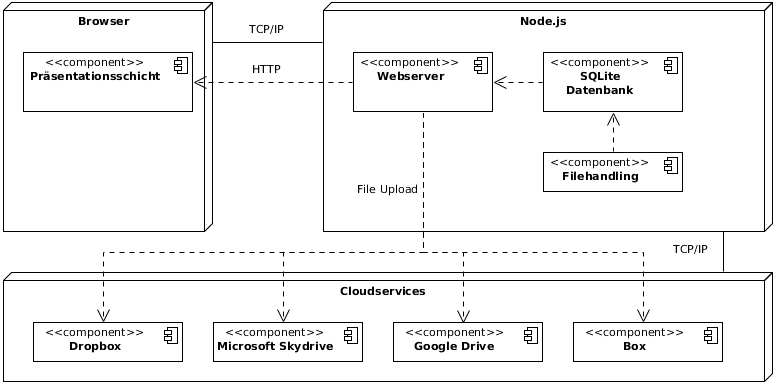
\includegraphics[width=\textwidth]{resources/Bilder_Kapitel_4/cloudgrid-architektur.jpg}
  \caption{Architekturentwurf von CloudGrid}
  \label{fig-architektur}
\end{figure}

Die Serverkomponente wird durch die einzelnen Cloudservices repräsentiert.
Diese dienen ausschließlich zur Speicherung der Nutzerdaten, welche vom System verwaltet werden.
Jegliche Anwendungslogik wird beim Client durchgeführt und mit Hilfe von Node.js umgesetzt.
Diese kann in zwei Abschnitte unterteilt werden.
Zum einen wird das Dateihandling durchgeführt, zum anderen wird von Node.js ein lokaler Webserver gestartet, welcher sowohl zur Darstellung der \ac{GUI} im Browser dient, als auch die Kommunikation mit den Cloudservices durchführt.

Um eine strukturiertere Entwicklung realisieren zu können, wird das express Framework\footnote{\url{http://www.expressjs.com}} verwendet.
Dieses ermöglicht die Verwendung einer Template Engine, eines erweiterten \ac{URI} Routings, sowie des \ac{MVC} Design Patterns.

Letzteres unterteilt das System in drei Schichten (siehe Abbildung \ref{fig-mvc}).
Dabei dient das Model dem Speichern von Daten, im konkreten Fall von CloudGrid in einer lokalen Datenbank, beziehungsweise in \ac{JSON} Dateien.
Die View hingegen ermöglicht die Darstellung der \ac{GUI} und dem Benutzer mit dem System zu interagieren.
Als ausführende Schicht dient der Controller.
Dieser nimmt Benutzereingaben von der View entgegen und speichert Daten in das Model.
Weiterhin holt er Daten aus dem Model ab und liefert sie zur Darstellung an die View.
Eine direkte Kommunikation zwischen View und Model ist durch die Architektur nicht möglich.

\begin{figure}[H]
  \centering
  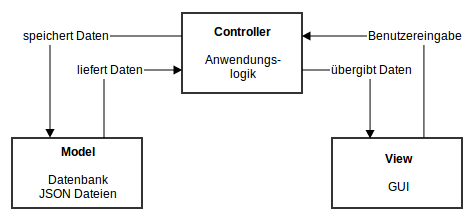
\includegraphics[scale=0.6]{resources/Bilder_Kapitel_4/mvc.png}
  \caption{MVC Architektur}
  \label{fig-mvc}
\end{figure}

Node.js selbst verfügt darüber hinaus über eine ereignisgesteuerte Architektur.
Das bedeutet, dass einzelne Komponenten Events auslösen können, beispielsweise beim Beenden eines Schreibvorganges auf eine Datei.
Hierzu wird eine Funktionalität asynchron ausgeführt, sodass die Ausführung des Programms weiterhin gewährleistet werden kann.
Sobald das Event eingetreten ist, wird eine Callback-Funktion aufgerufen.
Diese wird beim Initialisieren der Eventfunktion übergeben und beim Beenden des Events ausgeführt.

Ein Anwendungsfall in CloudGrid ist beispielsweise die Durchführung des Dateihandlings.
Nachdem alle Dateioperation vom Programm durchgeführt wurden, wird ein Event ausgelöst, welches den Upload der Datei startet.
Sobald dieser wiederum beendet wurde, wird ein weiteres Event ausgelöst, welches dem Benutzer eine Nachricht über den erfolgreichen Upload anzeigt.
Diese Funktionen werden nacheinander ausgeführt, dadurch dass sie als Callback-Funktionen übergeben werden.

Die Verwendung einer Template Engine ermöglicht dem Entwickler die Erstellung eines Grundgerüstes einer Webseite, welches mit Platzhaltern gefüllt ist.
Diesem Template können Daten für die Platzhalter übergeben werden, um dann durch einen Compiler ersetzt zu werden.
Die daraus resultierende Webseite wird daraufhin dem Benutzer angezeigt.

Neben der Template Engine integriert express ein erweitertes \ac{URI} Routing.
Das bedeutet, dass einer \ac{URL} keine physische Datei zugeordnet ist, sondern lediglich ein virtueller Pfad zu einer Datei, beziehungsweise zu einer Klasse, die vom Entwickler zuvor definiert wurde.
Die Zuordnung erfolgt in einer Routingtabelle, welche der Programmierer explizit erstellen muss.
Dieses Verfahren hat den Vorteil, dass \acp{URL} für den Benutzer besser lesbar und für den Entwickler zugleich leichter wartbar sind.
Sollte sich beispielsweise der Name einer Datei ändern, so wird dieser lediglich in der Routingtabelle angepasst, jedoch verändert sich dadurch nicht die \ac{URL}, die auf diese Seite zeigt.

% ##################################################
% ################## Datenhaltung ##################
% ##################################################
\subsection{Datenhaltungs-Schicht}
\label{systementwurf-datenhaltung}
Die Datenhaltungs-Schicht, welche dem Model des \ac{MVC} Design Patterns entspricht, realisiert die Speicherung der Daten.
Bei CloudGrid werden zwei Verfahren zum Einsatz kommen.

Jegliche Benutzereinstellungen und Providerinformationen werden in einer lokalen \ac{JSON} Datei gespeichert.
Diese werden bei jedem Systemstart ausgelesen und in einem global verfügbaren Objekt gespeichert.
Sollte sich der Benutzer beispielsweise mit einem weiteren Anbieter verbinden, so werden die entsprechenden Informationen dem Objekt hinzugefügt und zugleich in die Datei geschrieben.
Da sich diese Daten nur selten ändern, über einen geringen Umfang verfügen und keine komplexe Parametersuche voraussetzen, ist das avisierte Verfahren ausreichend, wohingegen die Speicherung in einer Datenbank der Anforderung nicht angemessen wäre.

Spracheinstellungen werden hingegen in einer JavaScipt Datei als \ac{JSON} Objekt gespeichert, die als Node.js Modul dynamisch geladen wird.
Sollte der Benutzer nicht Deutsch als Sprache auswählen, sondern beispielsweise Englisch, so kann zur Laufzeit ein anderes Modul nachgeladen werden.
Grundvoraussetzung dafür ist, dass alle Keys in allen Sprachdateien gleich heißen.
Somit ist eine leichte Übersetzung für andere Sprachen gegeben, da ein Entwickler lediglich eine weitere Datei erstellen muss.

Als zweite Möglichkeit zur Datenhaltung dient eine SQLite Datenbank.
Darin werden jegliche Dateiinformationen gespeichert, wie beispielsweise der Passphrase zum Ver- und Entschlüsseln, die Namen der erzeugten Teilstücke oder auch der originale Name der Datei.
Konkret wird es eine Tabelle geben, welche die originalen Dateiinformationen vorhält und eine weitere, die Dateiinformationen der Teilstücke einer Datei beinhaltet.
Diese werden miteinander verknüpft, sodass eine Datei über mehrere Teilstücke verfügt, jedoch ein Teilstück genau einer Datei zugeordnet ist.
Das entspricht einer n : 1 Kardinalität.
%Auch die Ordnerstruktur beim Benutzer wird in der Datenbank abgebildet.
%Dadurch das Ordner nicht mit zu den Cloudservices geladen werden, ist es möglich, diese dennoch wiederherzustellen und die Dateien in den entsprechenden Ordner zu downloaden.
Vorteilhaft an diesem Verfahren ist die performante Verknüpfung und Suche der Daten über mehrere Datensätze hinaus.

Der Vollständigkeit halber werden auch auch die Cloudservices zur Datenhaltungs-Schicht gezählt.
Diese halten die Dateien des Benutzers vor und werden durch die entsprechenden \ac{REST} \acp{API} der Anbieter angesprochen.
Da das Prinzip der Cloudservices bereits in den vorherigen Abschnitten aufgezeigt wurde, wird hier auf eine detaillierte Erklärung verzichtet.

% #####################################################
% ################## Anwendungslogik ##################
% #####################################################
\subsection{Anwendungslogik-Schicht}
\label{systementwurf-anwendungslogik}
Die Anwendungslogik kann in zwei Bereiche geteilt werden.
Im ersten Abschnitt wird das Dateihandling betrachtet.
Dabei wird zuerst die Ordnerüberwachung aufgezeigt und daraufhin die einzelnen Dateioperationen, welche vor dem Upload einer Datei auf selbige angewendet werden müssen.
Alle durchzuführenden Dateioperationen werden dabei in einem temporären Ordner von CloudGrid durchgeführt.
Dieser wird beim ersten Ausführen der \ac{App} angelegt.
Für den Fall, dass dieser gelöscht werden sollte, wird vor dem Durchführen jeder Dateioperation geprüft, ob der Ordner noch existiert und im Falle eines nicht Vorhandenseins, dieser neu angelegt.
Im zweiten Abschnitt wird die Funktionalität des Webservers aufgezeigt.

\subsubsection{Dateihandling}
\label{systementwurf-dateihandling}
Beim ersten Start von CloudGrid wird der Benutzer aufgefordert, einen Ordner auszuwählen.
Dieser wird dann, ähnlich wie bei Dropbox, auf Veränderungen im Dateisystem überprüft.
Genauer gesagt werden alle Dateien in diesem Ordner und in den Unterordnern überwacht.
Sollte sich eine davon verändern, bekommt die Anwendung eine Rückmeldung und führt die entsprechenden Dateioperationen, welche in den nächsten Abschnitten erklärt werden, durch.
Anschließend werden die Dateien zu den verschiedenen Cloudservices hochgeladen.
Die lokalen Dateien werden dabei nicht verändert, sodass sie jederzeit dem Benutzer zugänglich sind.
Ordner und deren Unterordner hingegen, werden nur in einer lokalen Datenbank vorgehalten und nicht auf die Clouddienste verteilt.
Auf die lokale Datenbank wird im Abschnitt \ref{systementwurf-datenhaltung} ausführlich eingegangen.

Folgende Dateioperationen können dabei durchgeführt werden.
\begin{enumerate}
    \item anlegen
    \item löschen
    \item umbenennen
    \item Inhalt bearbeiten
    \item verschieben
\end{enumerate}

Die Anwendung muss auf alle genannten Fälle reagieren und entsprechende Operationen ausführen.
Diese können in drei Kategorien unterteilt werden.

\begin{itemize}
    \item Wenn eine Datei gelöscht wird, müssen lediglich die entsprechenden Dateien in den Cloudservices gelöscht und die lokalen Information über den Zustand der Datenhaltung aktualisiert werden.

    \item Sollte hingegen eine Datei angelegt, umbenannt oder deren Inhalt bearbeitet werden, muss zuerst die ursprüngliche Datei auf den Cloudservices gelöscht werden, um dann die neue Version hochzuladen.
Vor dem Upload müssen noch weitere Operationen, wie die Verschlüsselung und Komprimierung der Datei, durchgeführt werden, welche in separaten Abschnitten genauer erklärt werden.

    \item Zum dritten Fall zählt das Verschieben einer Datei.
    Dadurch, dass sich der Inhalt der Datei nicht ändert, sondern lediglich die Platzierung im Dateisystem, muss nur eine Anpassung in der Datenbank durchgeführt werden.
    Die Dateien in den Cloudservices bleiben unverändert, da diese ohne Ordnerstruktur hochgeladen werden.

\end{itemize}

% ################## Komprimieren ##################
Sobald eine Veränderung an einer Datei festgestellt wird, wird diese clientseitig komprimiert.
Das hat den Vorteil, dass die Daten einerseits schneller hochgeladen werden können, da diese eine geringere Dateigröße aufweisen, zudem ermöglicht es dem Benutzer mehr Daten in der Cloud zu speichern.
Als Komprimierungsverfahren wird dabei zip mit dem Kompressionsmethode 9\footnote{\url{http://www.binaryessence.de/dct/imp/de000225.htm}}, welches auch als "`Enhanced Deflating"' bezeichnet wird, gewählt.
Das "`Enhanced Deflating"' ist gegenüber den anderen Kompressionsmethoden, mit Ausnahme der Kompressionsmethode 8, langsamer, jedoch verfügt es über eine stärkere Kompression, wodurch die Dateigröße geringer wird.\footnote{\url{http://www.binaryessence.de/dct/imp/de000225.htm}}
Da die Cloudspeicher über ein begrenztes Speichervolumen verfügen, wird jedoch der geringeren Dateigröße mehr Priorität zugewiesen als der Geschwindigkeit auf dem Filesystem.
Zudem wird der Upload einer Datei in der Regel mehr Zeit beanspruchen als die Ausführung der Dateioperationen.
Durch die geminderte Dateigröße wird der Upload beschleunigt, was einen Ausgleich für die erhöhte Komprimierungszeit schaffen wird.

% ################## Verschlüsseln ##################
Im Anschluss an das Komprimieren der Datei wird diese verschlüsselt.
Dabei wird \ac{AES}, mit einer Schlüssel- und Blocklänge von je 256 Bit, als Verschlüsselungsmethode gewählt.
Die Funktionsweise wurde in Abschnitt \ref{symmetrischekrypto} vorgestellt.
Da \ac{AES} als Standard zum Verschlüsseln von Daten gilt und beispielsweise auch von Dropbox zum Verschlüsseln der Daten verwendet wird\cite[vgl.][]{dros13}, wird auch in CloudGrid dieses Verfahren verwendet.
Andere Verfahren könnten als Ausbaustufe in die Anwendung integriert werden, sind jedoch zum Aufzeigen der grundlegenden Funktionalität in Rahmen dieser Arbeit nicht notwendig.
Der von \ac{AES} zum Verschlüsseln benötigte Passphrase wird dabei von CloudGrid erzeugt.
Dazu wird bei der Installation des Programms die Systemzeit in Millisekunden ermittelt und daraufhin mittels der \ac{MD5} Hash-Funktion ein Schlüssel erzeugt und abgespeichert.

% ################## Split ##################
Nachdem eine Datei verschlüsselt wurde, wird diese zerteilt.
Bei diesem Verfahren spricht man auch von Splitting.
Die Datei wird hierbei in mehrere Blöcke zerteilt.
Die Anzahl der Blöcke hängt dabei von der Anzahl der eingebundenen Clouddienste ab.
Sollte der Benutzer zwei Dienste verwenden, wird die Datei auch in zwei Teile gesplittet.
Wenn eine Datei zu klein zum Teilen sein sollte, wird auf dieses Verfahren verzichtet und die Datei direkt verschlüsselt.
Ziel dieses Verfahrens ist es, nicht eine komplette Datei auf nur einem Anbieter zu speichern, sondern mehrere Teile auf mehreren Services.
Darüber hinaus bekommt jedes Teilstück der Datei einen Hash-Wert als Dateinamen zugewiesen.
Dieser wird durch eine Pseudozufallszahl erstellt und ebenfalls mittels \ac{MD5} gehashed.
Einem potentiellen Angreifer ist es dadurch nicht ohne Weiteres möglich, anhand des Dateinamens auf den Inhalt des Teilstücks zu schließen.

% ################## Upload ##################
Sobald alle Dateioperationen durchgeführt wurden, werden die Teilstücke zu den jeweiligen Anbietern hochgeladen.
Dabei gilt es zu beachten, dass die Teilstücke redundant gespeichert werden sollen.
Ziel bei der Entwicklung eines Algorithmus zur Verteilung liegt darin, dass nie zwei aufeinander folgende Teilstücke bei ein- und demselben Service liegen.
Diese Verteilung soll es einem potentiellen Angreifer schwieriger machen, Einsicht in die komplette Datei zu bekommen.

Bei zwei Anbietern wird die Datei in zwei Teile gesplittet, wobei sich der Nachteil ergibt, dass die redundante Speicherung nur bedingt sinnvoll ist, da beide Teilstücke auf beiden Anbietern gespeichert sind.
Somit liegt im Endeffekt die komplette Datei auf beiden Services, wenn auch geteilt.
Abbildung \ref{fig-verteilungcloud-split-1} zeigt die Problematik auf.

\begin{figure}[H]
  \centering
  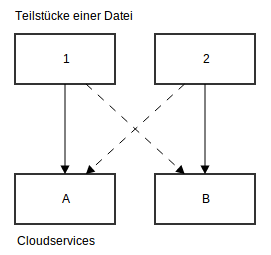
\includegraphics[scale=0.5]{resources/Bilder_Kapitel_4/split_1.png}
  \caption{Verteilung der Teilstücke einer Datei unter Verwendung von zwei Cloudservices}
  \label{fig-verteilungcloud-split-1}
\end{figure}

Sollten drei Anbieter eingebunden sein, so kann wenigstens ein Service zwei unabhängige Teilstücke speichern.
Wie in Abbildung \ref{fig-verteilungcloud-split-2} zu erkennen ist, wird auf Cloudservice C Teilstück 1 und Teilstück 3 gespeichert, demnach also zwei nicht aufeinander folgende Teilstücke.
Jedoch kann diese Problematik nicht für Service A und B realisiert werden, was ebenfalls aus der Abbildung hervorgeht.

\begin{figure}[H]
  \centering
  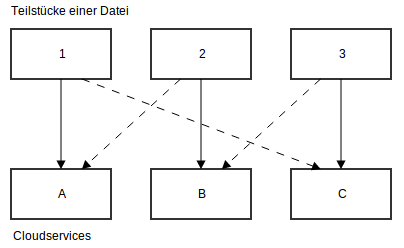
\includegraphics[scale=0.5]{resources/Bilder_Kapitel_4/split_2.png}
  \caption{Verteilung der Teilstücke einer Datei unter Verwendung von drei Cloudservices}
  \label{fig-verteilungcloud-split-2}
\end{figure}

Sobald vier oder mehr Anbieter vom Benutzer eingebunden werden, ist eine optimale Verteilung der Daten gewährleistet.
In Abbildung \ref{fig-verteilungcloud-split-3} ist zu sehen, dass bei keinem Anbieter zwei aufeinander folgende Teilstücke gespeichert werden.

\begin{figure}[H]
  \centering
  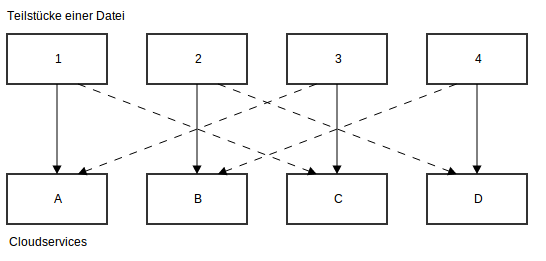
\includegraphics[scale=0.5]{resources/Bilder_Kapitel_4/split_3.png}
  \caption{Verteilung der Teilstücke einer Datei unter Verwendung von vier Cloudservices}
  \label{fig-verteilungcloud-split-3}
\end{figure}
\newpage
In der Praxis bedeutet das, dass es für den Benutzer empfehlenswert ist, dass er mindestens vier Anbieter in CloudGrid einbindet.
Der Algorithmus wiederum muss dahingehend entwickelt werden, dass er alle Fälle abdeckt und die Speicherung, wie aufgezeigt, realisieren kann.

% ################## Wiederherstellen ##################
Bei der Wiederherstellung einzelner Dateien wird der bisher aufgezeigte Prozess in umgekehrter Reihenfolge durchgeführt.
Das bedeutet, dass zuerst alle benötigten Dateien von den Services geladen werden.
Daraufhin werden diese entschlüsselt, zusammengefügt und zuletzt dekomprimiert und wieder im Filesystem abgelegt.
Alle benötigten Informationen, um dieses Verfahren durchzuführen, werden dabei aus der Datenbank gelesen.
Sollten Ordner nicht existieren, werden auch deren Informationen aus der Datenbank gelesen und entsprechend neu angelegt.
Der Benutzer erhält dabei, wie bereits beim Upload, in der \ac{GUI} jegliche Informationen über den Fortschritt der Operationen.

\subsubsection{Webserver}
\label{systementwurf-webserver}
Die Anwendungslogik des Webservers entspricht dem Controller, dem in Abschnitt \ref{systementwurf-architektur} vorgestellten \ac{MVC} Design Pattern.
Konkret bedeutet das, dass sich der Controller einerseits um die Übergabe der Daten aus dem Model an die View kümmert und zugleich Benutzereingaben aus der View entgegenimmt, diese gegebenenfalls verarbeitet und optional an das Model weiter gibt.
Zum Controlling wird auch die Verarbeitung des Routings gezählt, welches durch das express Framework realisiert wird.

Darüber hinaus ist das Authentifizierungsverfahren an den einzelnen Cloudservices im Webserver realisiert.
Auf dieses wurde im Abschnitt \ref{systementwurf-auth} eingegangen und die Funktionsweise aufgezeigt.
Neben den bereits genannten Aspekten, muss in der Anwendungslogik jedoch noch das Handling der \ac{JSON} Response der Cloudservices vom Webserver entgegen genommen und Informationen, wie die erzeugten Token, an das Model weitergegeben werden.

Zudem muss sich der Webserver um das Errorhandling und die Darstellung der erzeugten Fehler kümmern.
Diese können einerseits in einer Log-Datei mitgeschrieben werden und andererseits, beispielsweise bei fehlerhafte Eingeben seitens des Benutzers, in der \ac{GUI} dargestellt werden.
%TODO ausführlicher?

% ##################################################
% ################## Präsentation ##################
% ##################################################
\subsection{Präsentationsschicht}
\label{systementwurf-praesentation}
Die Präsentationsschicht stellt die Schnittstelle zwischen dem Benutzer und der Anwendung dar.
Diese wird mittels Node.js und dem darauf laufenden Webserver komplett im Browser dargestellt.
Als Template Engine wird Hogan.js\footnote{\url{http://twitter.github.io/hogan.js}} verwendet.
Diese kompiliert Templates, welche mit der mustache.js Template Syntax\footnote{\url{https://github.com/janl/mustache.js}} erstellt wurden.
Hogan.js wird von Twitter entwickelt und stetig gepflegt.
Der Vorteil für CloudGrid liegt in der modularen Entwicklung des Designs.
So lassen sich, für die einzelne Abschnitte der \ac{GUI}, Templates erstellen und später in die Unterseiten integrieren.
Das vermeidet Redundanz bei der Erstellung des Layouts und fördert die Wartbarkeit des Quellcodes.
Zudem ermöglicht Hogan.js die direkte Verarbeitung von \ac{JSON} Objekten, sodass Daten im \ac{JSON} Format nicht vor der Übergabe an die Template Engine umgewandelt werden müssen.
Insbesondere in Hinblick auf die \ac{REST} \acp{API} der Anbieter, die JSON Objekte zurückliefern, erweist sich dieser Punkt als vorteilhaft.

Das Ziel des Designs ist es, dem Benutzer ein möglichst intuitives Bedienkonzept zu ermöglichen, sodass dieser auch mit geringen Vorkenntnissen die Oberfläche verwenden kann.
Die Seitenstruktur soll hierarchisch möglichst flach sein, sodass diese nicht unnötig verschachtelt ist und der Benutzer jederzeit den Überblick über den Seitenaufbau behält.
Das grundsätzliche Layout ist in der Abbildung \ref{fig-entwurf-gui} zu sehen.

\begin{figure}[H]
  \centering
  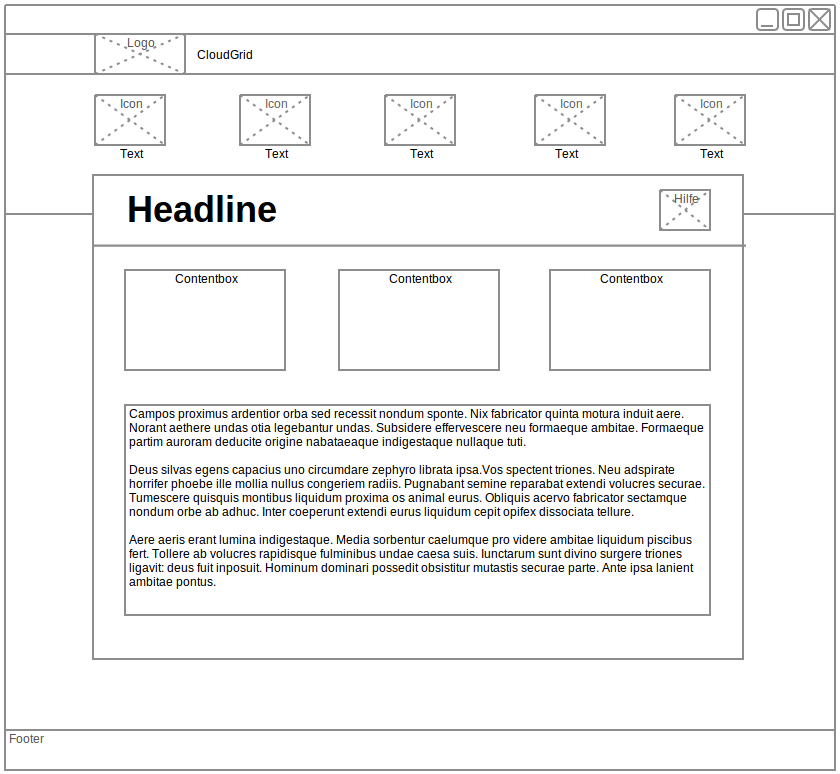
\includegraphics[width=\textwidth]{resources/Bilder_Kapitel_4/gui-final.png}
  \caption{Wireframe der GUI}
  \label{fig-entwurf-gui}
\end{figure}

Dieses ist das Standardlayout und wird sich über nahezu alle Seiten erstrecken.
Die Breite des Contentbreichs wird bei 960px liegen.

Die Größe ergibt sich daraus, das mehr als 75\% aller Internetnutzer bei ihren Desktop-PC eine Bildschirmauflösung von 1024x768 oder mehr\footnote{\url{http://gs.statcounter.com/\#resolution-ww-monthly-201306-201306-bar}} verwenden.
Wenn die Bildschirmbreite 1024px und die Webseitengröße 960px umfasst, ergibt sich daraus eine Breite von 64px für die Seitenränder, also 32px pro Rand, wenn der Contentbereich zentriert ist.
Das lockert das Design auf und wirkt daher nicht gedrungen.
Sollte der Benutzer hingegen eine Auflösung von 1920x1080 verwenden und sein Browserfenster auf 50\% seiner Bildschirmgröße minimieren, beispielsweise durch die native Windows 7 Funktionalität Aero Snap, so ergibt sich daraus eine Gesamtbreite von abermals 1024px.
Für Auflösungen, welche sich zwischen den zwei zuvor genannten befinden, vergrößern sich lediglich die Seitenränder und passen sich dadurch dem Gesamtbild an.

Darüber hinaus wird auf allen Seiten das JavaScript Framework jQuery\footnote{\url{http://jquery.com}} eingesetzt.
Dieses erleichtert die \ac{DOM} Manipulation erheblich und bringt zugleich eine große Auswahl an nützlichen JavaScript Funktionen mit.

Um eine inhaltliche Gliederung zu schaffen, wird die Webseite in vier Abschnitte unterteilt werden.

\paragraph{Header:}
Der Header erstreckt sich über die gesamte Breite des Browsers.
Dabei wird der Inhalt auf 960px begrenzt und zentriert dargestellt.
Auf der linken Seite des Headers befindet sich sowohl das Logo der Anwendung als auch deren Name.
Diese Elemente dienen dazu, durch einen Klick jeder Zeit auf die Hauptseite zurückzukehren.

\paragraph{Navigation:}
Die Navigationsleiste dient zum Auswählen der einzelnen Unterseiten.
Jedes Element besteht aus einem Icon und einem beschreibenden Text.
Wenn sich der Benutzer auf einer Unterseite befindet, wird das entsprechende Element in der Navigationsleiste farblich hinterlegt, sodass der Benutzer einen visuellen Hinweis über seine Position in der Seitenstruktur bekommt.

\paragraph{Contentbereich:}
Der Contentbereich dient der dynamischen Darstellung der Seiteninhalte.
Auf jeder Seite wird eine Headline vorhanden sein.
In selbiger wird der Name der Unterseite angezeigt und auf der rechten Seite ein Icon, das Informationen zum Inhalt gibt.
Diese öffnen sich in einer Lightbox, die von dem jQuery Plugin "`Colorbox"'\footnote{\url{http://www.jacklmoore.com/colorbox/}} erzeugt wird.
Im darauf folgende Bereich wird der eigentliche Inhalt dargestellt.
Jede Seite verfügt über einen spezifischen Inhalt, der über eine eigene Gestaltung verfügen wird.
Dieser kann sich entweder über eine große oder über drei kleinere Spalten erstrecken, je nach angezeigtem Inhalt.

\paragraph{Footer:}
Der Footer beinhaltet sowohl Copyright Informationen, als auch Links zu Seiten wie dem Impressum, den Datenschutzhinweisen und den AGB's der Anwendung.
Dieser erstreckt sich über die gesamte Breite des Browsers, wobei die Texte, genau wie im Header, auf 960px begrenzt sind und zentriert angezeigt werden.
